\section{Schaltalgebra}
\subsection{Rechenregeln}

\textbf{Allg. $\Rightarrow$ Punkt vor Strich oder $\cdot$ vor $+$}

	\begin{tabular}{llll}
		Verkn"upfung mit 0 & $ a + 0 = a $ & $ a \cdot 0 = 0 $ & $ a \oplus 0 = a $\\
		Verkn"upfung mit 1 & $ a + 1 = 1 $ & $ a \cdot 1 = a $ & $ a \oplus 1 = \overline{a} $ \\
		Verkn. mit sich selbst & $ a + a = a $ & $ a \cdot a = a $ & $ a \oplus a = 0 $ \\
		Verkn. mit Inversem & $ a + \overline{a} = 1 $ & $ a \cdot \overline{a} = 0 $ & $ a \oplus \overline{a} = 1 $ \\
		\\
		Kommutativgesetz & $ a + b = b + a $ & $ a \cdot b = b \cdot a $ & $ a \oplus b = b \oplus a $\\
		Assioziativgesetz & $ (a + b) + c = a + (b + c) $ & $ (a \cdot b) \cdot c = a \cdot (b \cdot c) $ & $ (a \oplus b) \oplus c = a \oplus (b \oplus c) $ \\
		Distributivgesetz & $ a \cdot (b + c) = (a \cdot b) + (a \cdot c) $ & $ a + (b \cdot c) = (a + b) \cdot (a + c) $ & $ a \cdot (b \oplus c) = (a \cdot b) \oplus (a \cdot c) $ \\	
		\end{tabular}
\subsection{Vereinfachungen}
\begin{tabular}{lllll}
	$ a + (a \cdot b) = a $ & $(a \cdot b) + (a \cdot \overline{b}) = a $ &\hspace{2.0cm} &
	$  (a \cdot\overline{b}) + b = a + b$ & $ (a \cdot \overline{b}) \oplus b = a + b $\\
	$  a \cdot (a + b) = a $ & $ (a + b) \cdot (a + \overline{b}) = a $ &\hspace{2.0cm}&
	$ (a + \overline{b}) \cdot b = a \cdot b $ &$(a \oplus \overline{b}) \cdot b = a \cdot b  $\\
\end{tabular}

\subsection{Shannon und DeMorgan}
\begin{multicols}{2}
	\textbf{DeMorgan}\\
	$a \cdot b = \overline{\overline{(a \cdot b)}}= \overline{(\overline{a} + \overline{b})}$\\
	$a + b =  \overline{\overline{(a + b)}}= \overline{(\overline{a} \cdot \overline{b})}$

	\textbf{Shanon} (Vereinfachter Demorgan)\\
	- alle Variablen negieren\\
	- alle Operatoren negieren ($+ \rightarrow \cdot / \cdot \rightarrow +$)\\
	- ganzer Ausdruck negieren
\end{multicols}
\begin{tabular}{lll}
	Ursprungsschaltung: & Shannon & DeMorgan\\
		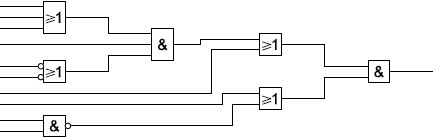
\includegraphics[width=0.3\textwidth]{pics/shanonursprung} & 
		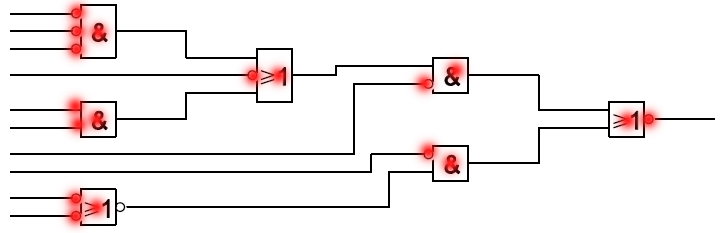
\includegraphics[width=0.3\textwidth]{pics/shanonende} &
		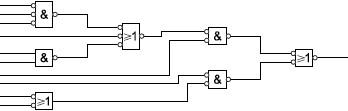
\includegraphics[width=0.3\textwidth]{pics/demorganende}\\
\end{tabular}


\subsection{Wahrheitstabelle, KDNF, KKNF}
\begin{multicols}{2}
\subsubsection{KDNF (Kanonisch  Disjunktive Normalform)}
\vspace{-5pt}
\textbf{Minterm}$~~$ \\
Zeile in WHT mit Funktionswert = \textbf{1}\\
$\rightarrow$ Eingangsvariablen AND($\cdot$)-Verknüpfen \\
$\rightarrow $ Eingangsvariable mit Wert \textbf{0} invertieren\\
\textbf{DNF (Sums of products)}\\
Minterme OR($+$)-Verknüpfen\\
\textbf{Kurzschreibweise:}\\
DNF: $ b = \#([1],[3],5) $ \\
Zahl entspricht Zeile, Eckige Klammern bedeutet don't care.\\ 

\subsubsection{KKNF (Kanonisch Konjunktive Normalform)}
\vspace{-5pt}
\textbf{Maxterm}$~~$ \\
Zeile in WHT mit Funktionswert = \textbf{0}\\
$\rightarrow$ Eingangsvariablen OR($+$)-Verknüpfen \\
$\rightarrow $ Eingangsvariable mit Wert \textbf{1} invertieren\\
\textbf{KNF (Products of sums)}\\
Maxterme AND($\cdot$)-Verknüpfen\\
\textbf{Kurzschreibweise:}\\
KNF: $ a = \&([1],[2],3) $ \\
Zahl entspricht Zeile, Eckige Klammern bedeutet don't care.\\ 

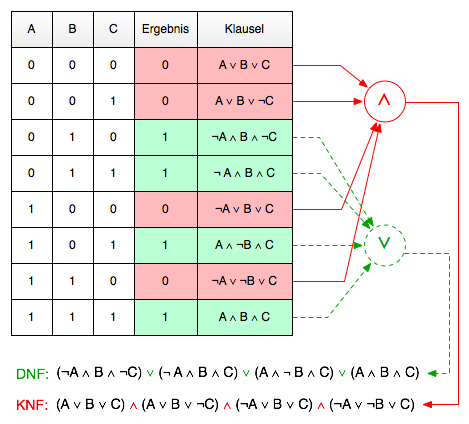
\includegraphics[width=0.5\textwidth]{pics/KNFDNF}
\end{multicols}

\subsection{Karnaugh-Diagramm}
\begin{tabular}{lll}
	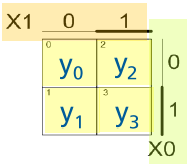
\includegraphics[width=0.1\textwidth]{pics/kv/2erKV} & 
	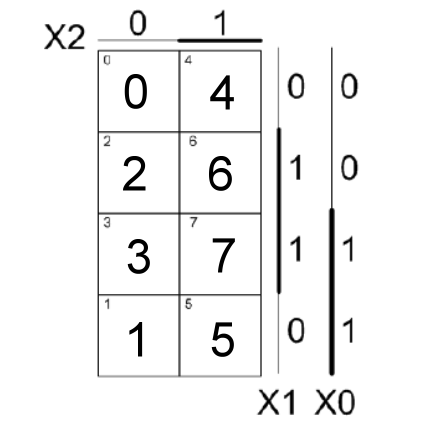
\includegraphics[width=0.1\textwidth]{pics/kv/3erKV} &
	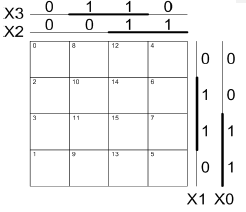
\includegraphics[width=0.15\textwidth]{pics/kv/4erKV}\\
\end{tabular}
\subsection{Arbeiten mit KV-Diagramm}
\begin{enumerate}
\setlength{\itemsep}{1pt}
  \setlength{\parskip}{0pt}
  \setlength{\parsep}{0pt}
\item Aufstellen der Wahrheitstabelle\\
\item "Ubertragen der Funktionswerte der Wahrheitstabelle in KV Diagramm\\
\item M"oglichst grosse Gruppen à $2^n$ Felder bilden\\
\begin{tabular}{|p{7cm}|p{7cm}}
	\textbf{DNF} & \textbf{KNF} \\
	Gruppen von Feldern mit Wert 1 oder d & Gruppen von Feldern mit Wert 0 oder d\\
\end{tabular}
\item Terme aus KV-Diagramm lesen\\
\begin{tabular}{|p{7cm}|p{7cm}}
	Variablen in Gruppe \textbf{AND}-Verknnüpfen & Variablen in Gruppe \textbf{OR}-Verknüpfen\\
	$\rightarrow$ \textbf{Variable = 0 invertieren}&$\rightarrow$ \textbf{Variable = 1 invertieren}\\
	\textbf{OR}-Verknüpfen aller Primimplikanten & \textbf{AND}-Verknüpfen aller Primimplikanten\\
\end{tabular}
\end{enumerate}